\documentclass[10pt,a4paper]{article}
\usepackage[latin1]{inputenc}
\usepackage{amsmath}
\usepackage{amsfonts}
\usepackage{amssymb}
\usepackage{graphicx}
\usepackage{amssymb}
\author{Paul Wieland}
\title{INF3490 Mandatory Assignment 2:
	Multilayer Perceptron}
\date{Deadline: Tuesday, October 16th, 2018 23:59:00}
\begin{document}
	\maketitle
	\tableofcontents
	\newpage
	%%%%%%%%%%%%%%%%%%%%%%%%%%%%%%%%%%%%%%%%%%%%%%%% 	%INTRODUCTION
	\section{Introduction}
	\subsection{Task}									%task
	We will build a Multilayer Perceptron to steer a robotic prosthetic hand. There are 40 inputs of electromyographic signals that we will classify. \\
	There are 8 classification values corresponding to a different hand motion: \\
	\begin{center}
		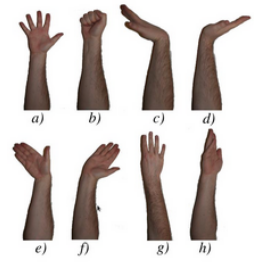
\includegraphics[width=0.4\linewidth]{pictures/hand}
		\\
		Possible motions \footnote{http://folk.uio.no/kyrrehg/pf/papers/glette-ahs08.pdf}
		\\
	\end{center}
	\begin{center}
		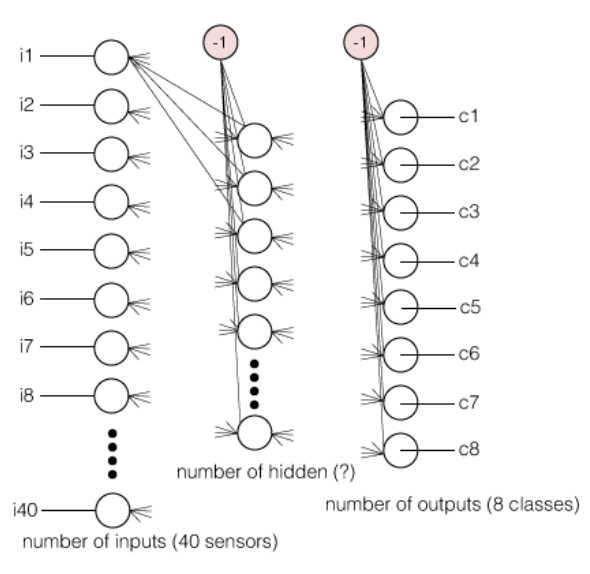
\includegraphics[width=0.7\linewidth]{pictures/mlp}
		\\
		Multilayer Perceptron for our problem \footnote{https://www.uio.no/studier/emner/matnat/ifi/INF3490/h18/assignments/assignment-2/assignment\_2.pdf}
		\\
	\end{center}
	We build a Multilayer Perceptron with 40 entry nodes, that means one node for each input. Then there is one hidden layer with a various number of hidden nodes. For classifying the input, there are 8 output nodes corresponding to the 8 hand motions. We only use one hidden layer to solve this problem.

	\subsection{Training Data}							%training data
	For each input vector:
	\begin{center}
		$ input = [i_1,i_2,i_3,i_4,...,i_{40}], i_n \in  \mathbb{R},n \in [40]  $
	\end{center}
	we have a target output vector:
	\begin{center}
		$ output = [c_1,c_2,c_3,c_4,...,c_8], c_n \in \{0,1\}, n \in [8],\sum_{n=1}^{8} c_n  = 1   $
	\end{center}
	That means, forwarding the input should result in the given target vector. 
	%%%%%%%%%%%%%%%%%%%%%%%%%%%%%%%%%%%%%%%%%%%%%%%%		%Implementation
	
\end{document}